\begin{itemize}
	
\item \textbf{Save User Route:}\\In this service contract, the code does obliged to all requested pertained in the conditions set out for this service contract. However the code does miss out on catering for the condition not stipulated which is the start saving a start point that is the same location as the end point.\\
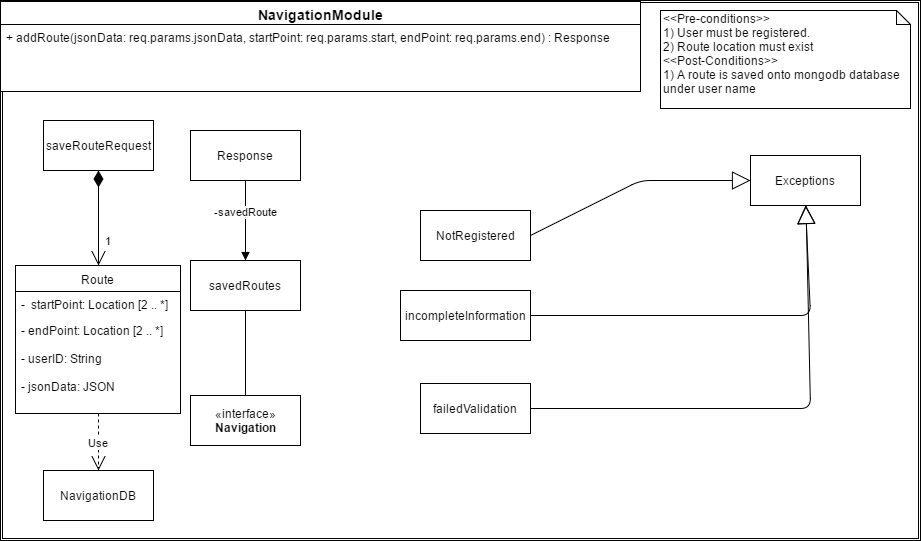
\includegraphics[scale=0.5]{SaveRoute.png}
\caption{Service Contract: Save User Route}
	\textbf{Mark: 8/10}
	
\item \textbf{Save User Preference:}\\Service contract requires to save different preferences to a specific user when all Pre-Conditions are met. In this test, A discovery was made whereby the request overrides already existing preferences instead of appending new preferences or throw an exception if preference is used. This thus leads to it not fully fulfilling the service contract stipulated.\\
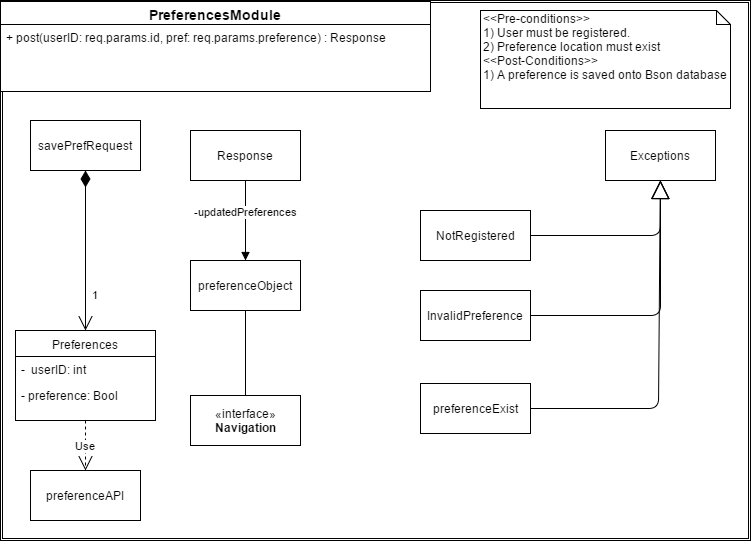
\includegraphics[scale=0.5]{SPrefServiceContract.png}
\caption{Service Contract: Save User Preference}
	\textbf{Mark: 4/10}
	
\item \textbf{Cache Routes:}\\In this service contract, routes that was saved onto cache is retrieved if route request exists in cache. In all test cases, the cache route is retrieved and if not, a request is made, this fulfills the service contract post condition. To thoroughly validate, we used Postman as an additional third party to validate POST request on database and cached file.\\
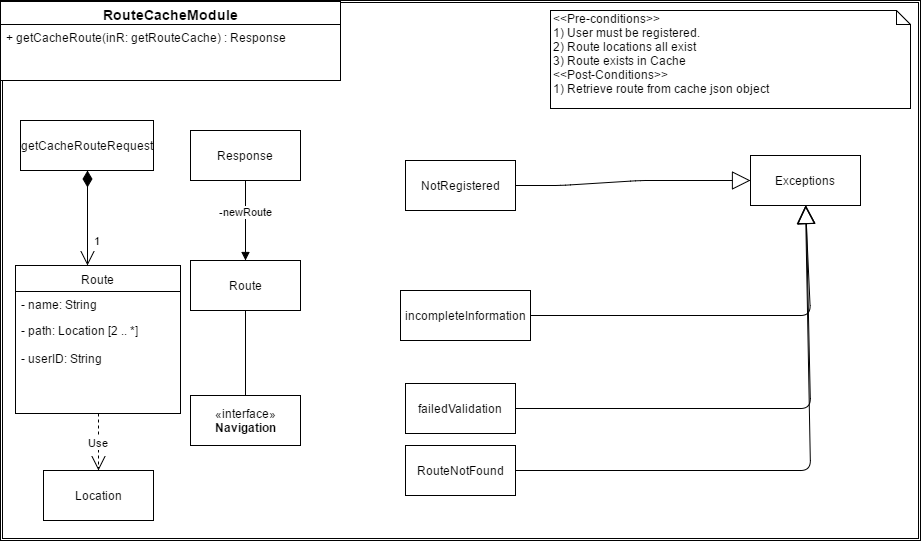
\includegraphics[scale=0.5]{CacheRoute.png}
\caption{Service Contract: Get Cache Route}
	\textbf{Mark: 9/10}
	
\end{itemize}